\section*{Experimental setup}
A program in MatLab was constructed to conduct the test with a \textit{Transformed 1-Up/2-Down Method}. A flowchart over the program can be seen in \autoref{app:Flowchart} and the script for the program is attached in the email under the name: "TransAdjustment.m". Other equipment used in the experimental setup is a pair of Bang $\&$ Olufsen H6 headphones and a Dell Latitude 6430u Ultrabook with a fixed 10 \% volume.

Two tones are presented to the test subject. The subject is then asked in the command window which of the two stimuli had the highest pitch. The subject is instructed to either enter "1" (for the first presented tone) or "2" (for the last presented tone) in the command window in MatLab.\blankline
%
\begin{figure}[H]
\centering
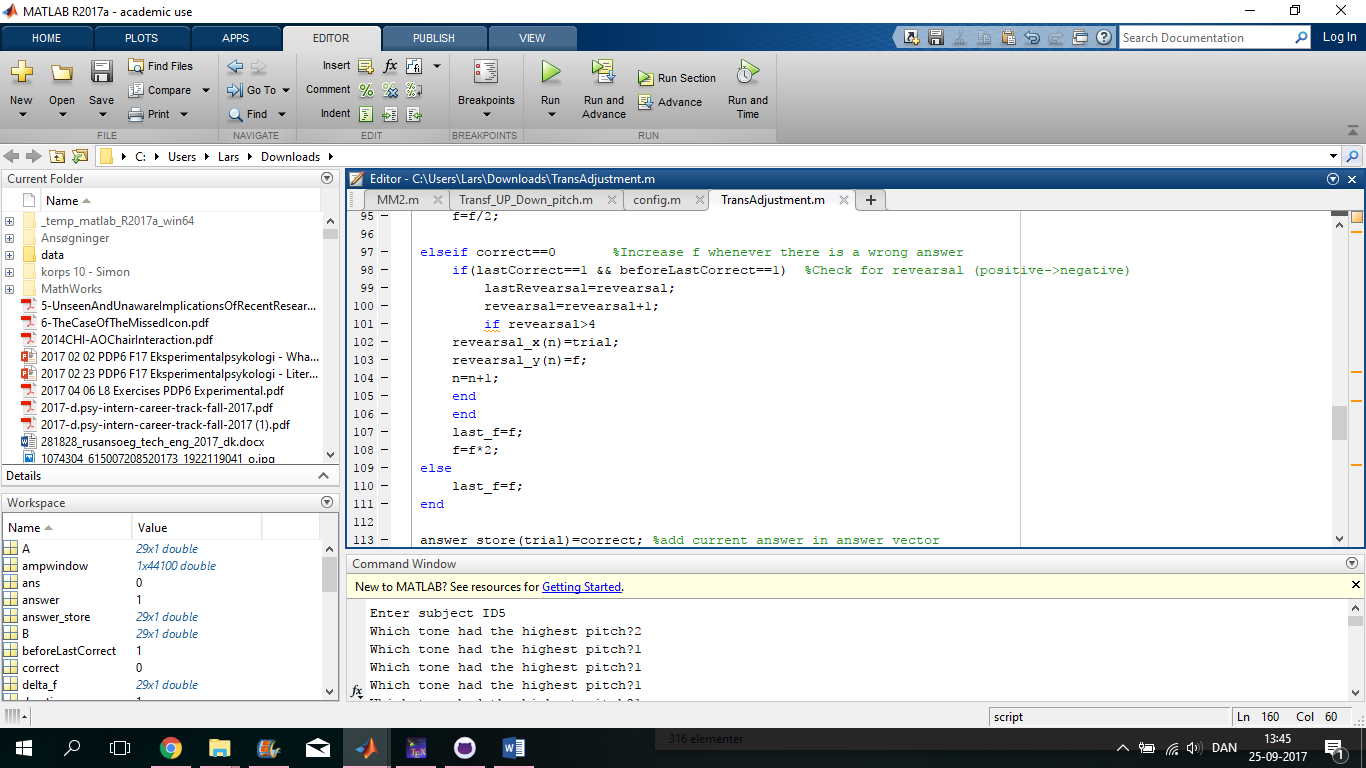
\includegraphics[width = 0.85\textwidth]{Figure/Interface.png} 
\caption{An illustration of the interface when it receives an answer from the test subject in the command window.}
\label{fig:TestInterface}
\end{figure}
\noindent
% 
The experiment was conducted in group room B2-207 located on the 1st floor of Fredrik Bajers vej 7B at Aalborg University and the test subjects were instructed to wear the headphones during the test and listen to the two tones. On \autoref{fig:experiment} the experimental setup is illustrated. 
%
\begin{figure}[H]
\centering
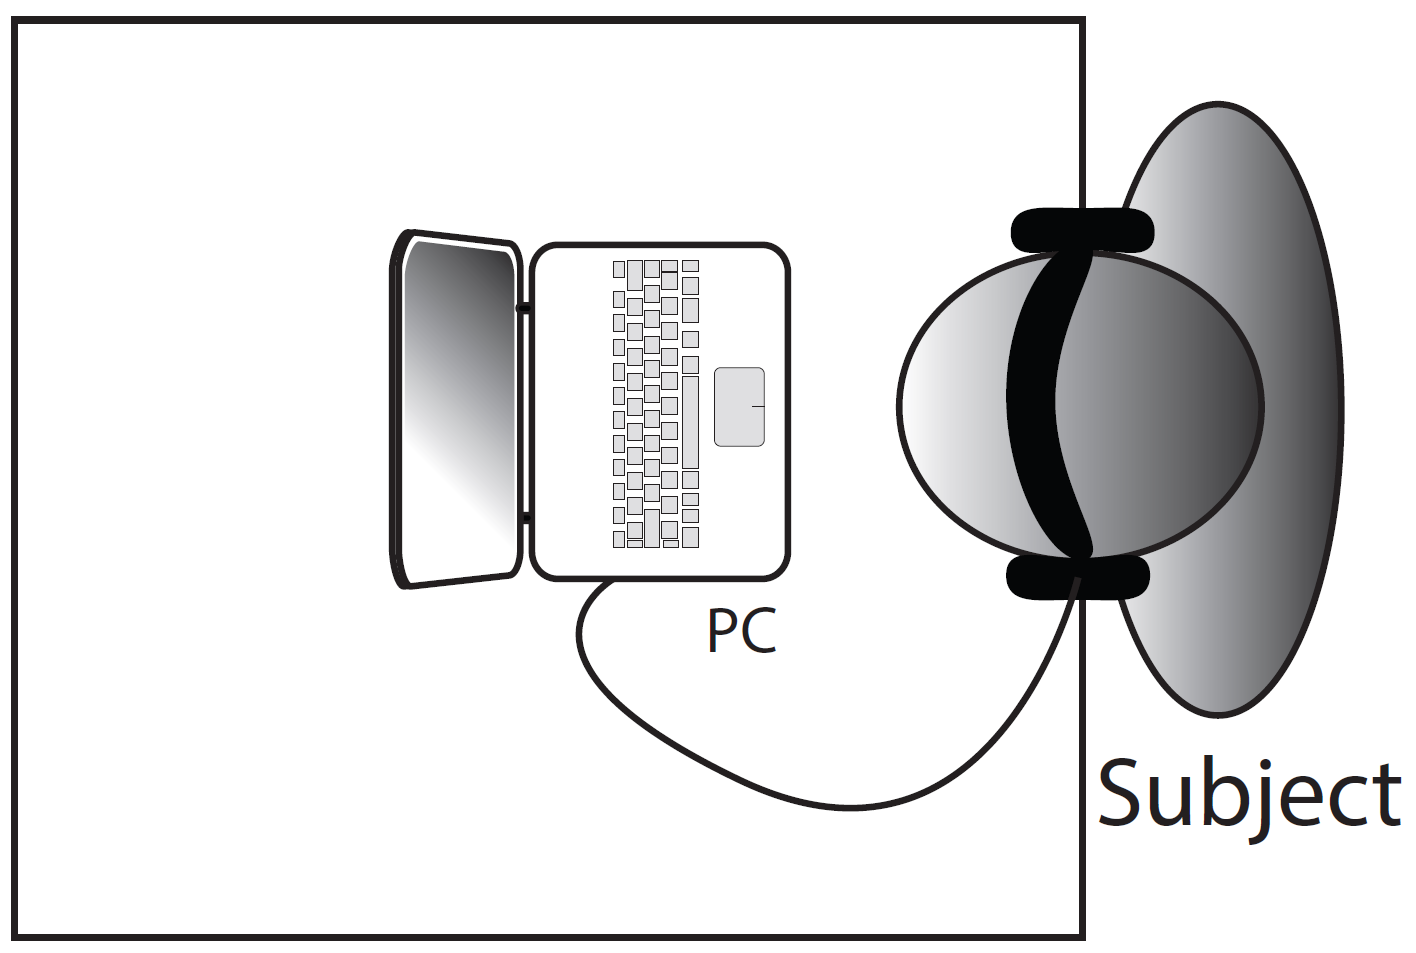
\includegraphics[width = 0.5\textwidth]{Figure/experiment.png} 
\caption{A sketch of the experimental setup.}
\label{fig:experiment}
\end{figure}
%

\subsection*{Test subjects}
%
Five test subjects were used in the test, two males and three females in the age of 23 to 24 (mean = 23.4). All of the test subjects are Engineering Psychology students at Aalborg University. 